%% IMPORTANT NOTICE:
%% 
%% For the copyright see the source file.
%% 
%% Any modified versions of this file must be renamed
%% with new filenames distinct from sample-sigconf.tex.
%% 
%% For distribution of the original source see the terms
%% for copying and modification in the file samples.dtx.
%% 
%% This generated file may be distributed as long as the
%% original source files, as listed above, are part of the
%% same distribution. (The sources need not necessarily be
%% in the same archive or directory.)
%%
%%
%% Commands for TeXCount
%TC:macro \cite [option:text,text]
%TC:macro \citep [option:text,text]
%TC:macro \citet [option:text,text]
%TC:envir table 0 1
%TC:envir table* 0 1
%TC:envir tabular [ignore] word
%TC:envir displaymath 0 word
%TC:envir math 0 word
%TC:envir comment 0 0
%%
%% The first command in your LaTeX source must be the \documentclass
%% command.
%%
%% For submission and review of your manuscript please change the
%% command to \documentclass[manuscript, screen, review]{acmart}.
%%
%% When submitting camera ready or to TAPS, please change the command
%% to \documentclass[sigconf]{acmart} or whichever template is required
%% for your publication.
%%
%%
\documentclass[sigconf]{acmart}
%%
%% \BibTeX command to typeset BibTeX logo in the docs
\AtBeginDocument{%
  \providecommand\BibTeX{{%
    Bib\TeX}}}

%% Rights management information.  This information is sent to you
%% when you complete the rights form.  These commands have SAMPLE
%% values in them; it is your responsibility as an author to replace
%% the commands and values with those provided to you when you
%% complete the rights form.
% \setcopyright{hotpotatolicense}
\copyrightyear{2024}
\acmYear{2024}
\acmDOI{5555555.5555555}
%% These commands are for a PROCEEDINGS abstract or paper.
\acmConference[WWU]{Bioinformatics Super Cool Conference}{December 4-5, 2024}{Bellingham, WA}
%%
%%  Uncomment \acmBooktitle if the title of the proceedings is different
%%  from ``Proceedings of ...''!
%%
%%\acmBooktitle{Woodstock '18: ACM Symposium on Neural Gaze Detection,
%%  June 03--05, 2018, Woodstock, NY}
% \acmISBN{978-1-4503-XXXX-X/18/06}


%%
%% Submission ID.
%% Use this when submitting an article to a sponsored event. You'll
%% receive a unique submission ID from the organizers
%% of the event, and this ID should be used as the parameter to this command.
%%\acmSubmissionID{123-A56-BU3}

%%
%% For managing citations, it is recommended to use bibliography
%% files in BibTeX format.
%%
%% You can then either use BibTeX with the ACM-Reference-Format style,
%% or BibLaTeX with the acmnumeric or acmauthoryear sytles, that include
%% support for advanced citation of software artefact from the
%% biblatex-software package, also separately available on CTAN.
%%
%% Look at the sample-*-biblatex.tex files for templates showcasing
%% the biblatex styles.
%%

%%
%% The majority of ACM publications use numbered citations and
%% references.  The command \citestyle{authoryear} switches to the
%% "author year" style.
%%
%% If you are preparing content for an event
%% sponsored by ACM SIGGRAPH, you must use the "author year" style of
%% citations and references.
%% Uncommenting
%% the next command will enable that style.
%%\citestyle{acmauthoryear}

\usepackage{graphicx}
\usepackage{subfig}
\usepackage{hyperref}

\begin{document}

\title{Automated Cell Structure Localization in Cellular Images}

%%
%% The "author" command and its associated commands are used to define
%% the authors and their affiliations.
%% Of note is the shared affiliation of the first two authors, and the
%% "authornote" and "authornotemark" commands
%% used to denote shared contribution to the research.
\author{Diego Llanes}
\email{fettigj@wwu.edu}
\email{wwu@diegollanes.com}
\affiliation{%
  \institution{Department of Computer Science, Western Washington University}
  \city{Bellingham}
  \state{Washington}
  \country{USA}
}

\author{Andrew Holmes}
\email{holmesa8@wwu.edu}
\affiliation{%
  \institution{Department of Computer Science, Western Washington University}
  \city{Bellingham}
  \state{Washington}
  \country{USA}
}

\author{AUTHOR}
\email{AUTHOR@wwu.edu}
\affiliation{%
  \institution{Department of Computer Science, Western Washington University}
  \city{Bellingham}
  \state{Washington}
  \country{USA}
}

\author{AUTHOR}
\email{AUTHOR@wwu.edu}
\affiliation{%
  \institution{Department of Computer Science, Western Washington University}
  \city{Bellingham}
  \state{Washington}
  \country{USA}
}

\author{AUTHOR}
\email{AUTHOR@wwu.edu}
\affiliation{%
  \institution{Department of Computer Science, Western Washington University}
  \city{Bellingham}
  \state{Washington}
  \country{USA}
}

\author{AUTHOR}
\email{AUTHOR@wwu.edu}
\affiliation{%
  \institution{Department of Computer Science, Western Washington University}
  \city{Bellingham}
  \state{Washington}
  \country{USA}
}

\author{Emily}
\email{AUTHOR@wwu.edu}
\affiliation{%
  \institution{Department of Biology, Western Washington University}
  \city{Bellingham}
  \state{Washington}
  \country{USA}
}

\author{Nick Galati}
\email{AUTHOR@wwu.edu}
\affiliation{%
  \institution{Department of Biology, Western Washington University}
  \city{Bellingham}
  \state{Washington}
  \country{USA}
}

\renewcommand{\shortauthors}{Llanes et al.}

\begin{abstract}
	Current cell microscopy labs manually stain mammalian tumor cells with antibodies in order to visually identify cell structures -- cilia, cilia base, and golgi apparatus. They are interested in the distance between the base of the cilia and the center of mass of the corresponding golgi apparatus. Measuring these distances requires manual labor and expert knowledge to accurately detect regions of interest and accurately decide the points in which to calculate a distance metric for. We propose a computer vision approach to automate this process. Our process involves: thresholding images of cells, clustering the points, and generating a convex hull around the clusters. We can then calculate a center of mass by integrating over the golgi apparatus and finding the intersection between the cilia and cilia base to determine the two points in which a distance metric can be calculated on.
\end{abstract}

%%
%% The code below is generated by the tool at http://dl.acm.org/ccs.cfm.
%% Please copy and paste the code instead of the example below.
%%
% \begin{CCSXML}
% <ccs2012>
%  <concept>
%   <concept_id>00000000.0000000.0000000</concept_id>
%   <concept_desc>Do Not Use This Code, Generate the Correct Terms for Your Paper</concept_desc>
%   <concept_significance>500</concept_significance>
%  </concept>
%  <concept>
%   <concept_id>00000000.00000000.00000000</concept_id>
%   <concept_desc>Do Not Use This Code, Generate the Correct Terms for Your Paper</concept_desc>
%   <concept_significance>300</concept_significance>
%  </concept>
%  <concept>
%   <concept_id>00000000.00000000.00000000</concept_id>
%   <concept_desc>Do Not Use This Code, Generate the Correct Terms for Your Paper</concept_desc>
%   <concept_significance>100</concept_significance>
%  </concept>
%  <concept>
%   <concept_id>00000000.00000000.00000000</concept_id>
%   <concept_desc>Do Not Use This Code, Generate the Correct Terms for Your Paper</concept_desc>
%   <concept_significance>100</concept_significance>
%  </concept>
% </ccs2012>
% \end{CCSXML}

% \ccsdesc[500]{Do Not Use This Code~Generate the Correct Terms for Your Paper}
% \ccsdesc[300]{Do Not Use This Code~Generate the Correct Terms for Your Paper}
% \ccsdesc{Do Not Use This Code~Generate the Correct Terms for Your Paper}
% \ccsdesc[100]{Do Not Use This Code~Generate the Correct Terms for Your Paper}

%%
%% Keywords. The author(s) should pick words that accurately describe
%% the work being presented. Separate the keywords with commas.
\keywords{Computer-Aided Microscopy, Cellular Localization, Biological Imaging, Object Detection}

% \received{20 February 2007}
% \received[revised]{12 March 2009}
% \received[accepted]{5 June 2009}

%%
%% This command processes the author and affiliation and title
%% information and builds the first part of the formatted document.
\maketitle

\section{Introduction}
\label{sec:intro}


\begin{figure}
	\centering
	\subfloat[Cilia Channel]{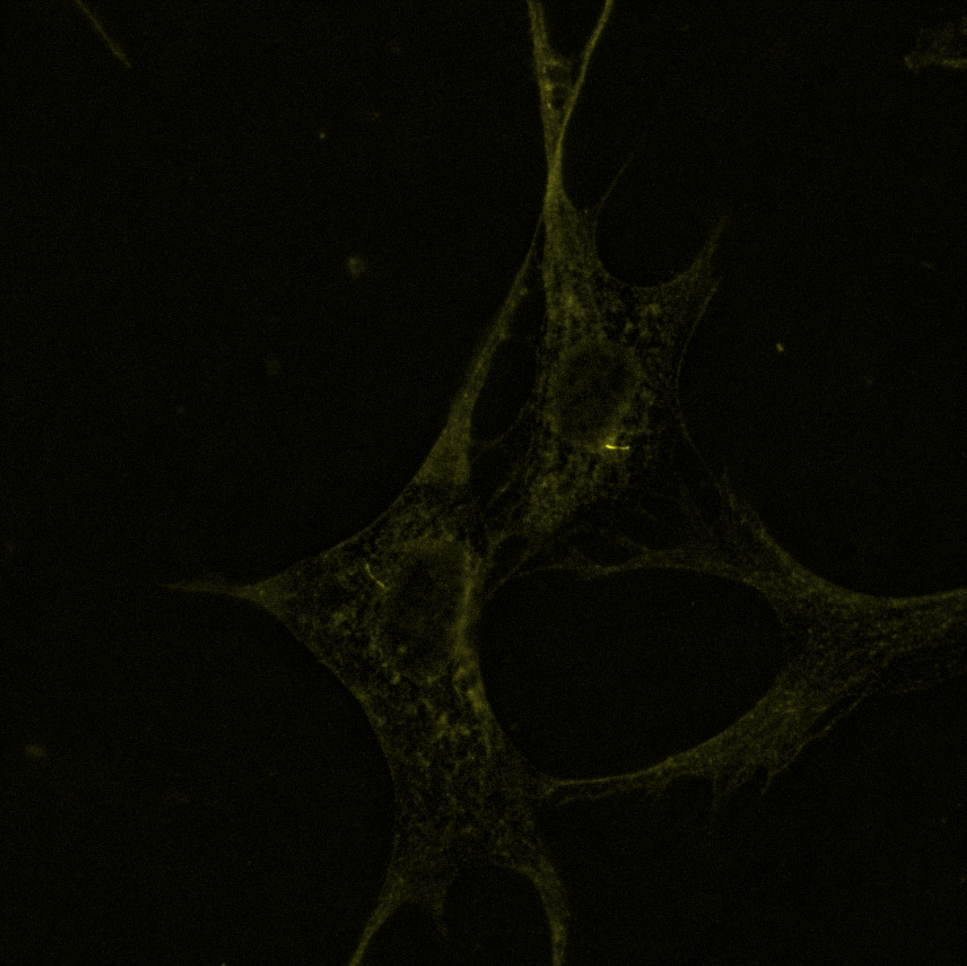
\includegraphics[width=0.3\linewidth]{figures/cilia.png}} \hfill
	\subfloat[Cilia Base Channel]{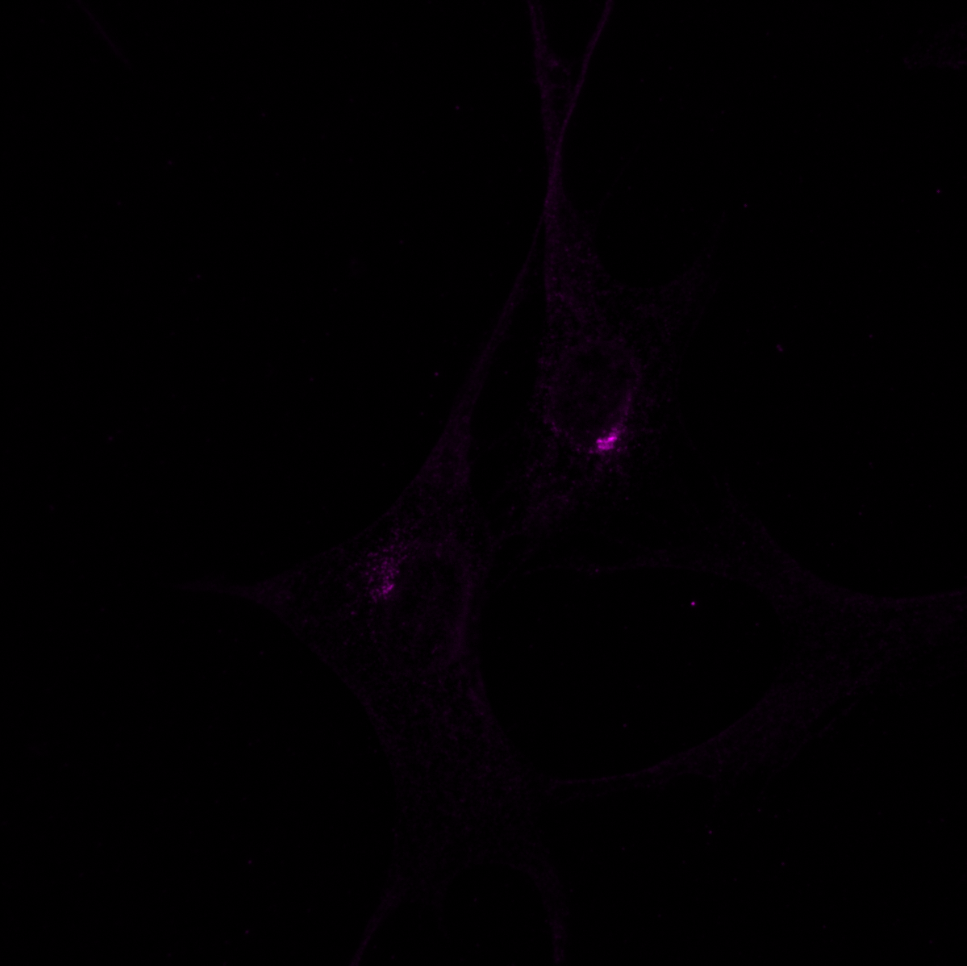
\includegraphics[width=0.3\linewidth]{figures/cilia_base.png}} \hfill
	\subfloat[Golgi Apparatus Channel]{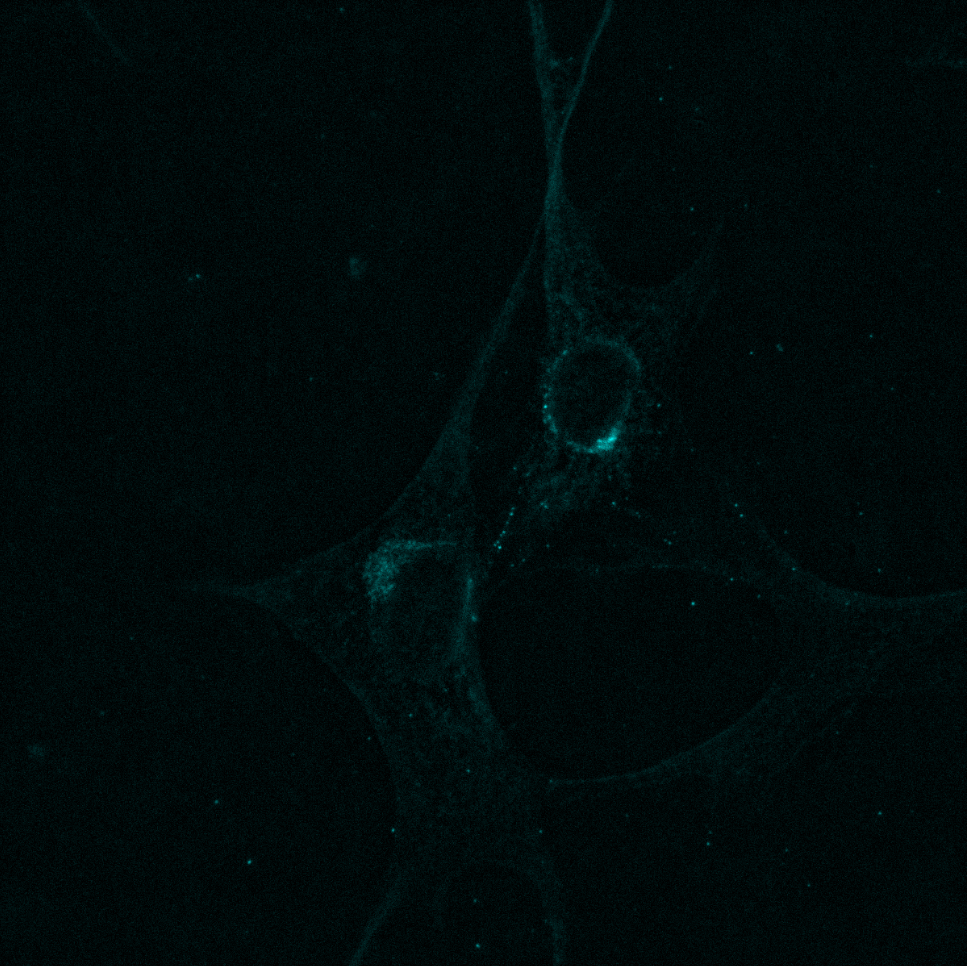
\includegraphics[width=0.3\linewidth]{figures/golgi.png}}
	\caption{shows three channels of the same scene that depicts two cells and the location of their cilia (left), cilia base (middle), and the golgi apparatus (right) through a process that stains specific regions of interest.}
\end{figure}

\section{Related Works}
\label{sec:background}

Put some background information here.

\section{Methods}
\label{sec:methods}

We are using computer vision techniques to threshold, cluster \cite{Ester1996ADA}, generate convex hull, and then calculate distances.

\subsection{Thresholding}
\label{sec:thresh}
\dots

\subsection{Distance Calculation}
\label{sec:dist}
\dots

\section{Results}
\label{sec:results}
\dots

\section{Conclusion}
\label{sec:conclusion}
\dots

\section(Next Steps}
\label{sec:future}
\dots



% Acknowledgments Section -- use (\acks)
\begin{acks}
We would like to acknowledge the Biology Department -- Professor Nick Galati and Emily LASTNAME -- for providing us with the data and helping us with the cross-disciplinary questions that we needed answered \dots
\end{acks}


\bibliographystyle{ACM-Reference-Format}
\bibliography{ref}


\end{document}
